% ------ headers globales y begin ---------------
\documentclass[11pt, a4paper, twoside]{article}
\usepackage{header_tp2}

\begin{document}{}

Para la medición de la performance del programa comparamos los tiempos en un caso aleatorio, un peor caso y 
un mejor caso, variando el tamaño de entrada ($n$ cantidad inicial de cartas). Además, quisimos comprobar que se 
cumpliera la cota teórica $\bigO{n^3}$ calculada. 

El algoritmo tiene una primera etapa de llenar la matriz calculando las mejor jugada para cada rango de cartas. Esta primera etapa es $\Theta(n^3)$.

Luego viene una última etapa de reconstruir la jugada que es $\Theta(cantidadDeTurnosDelJuego)$. Luego nos propusimos estudiar el comportamiento de nuestro algoritmo para distintas entradas, sabiendo que el peso principal de la complejidad no iba a ser afectado por el tipo de entrada, sino sólo por su tamaño. Dividimos los tipos de entrada en tres casos: 

\begin{itemize}
\item El caso $aleatorio$ se armó tomando valores generados de forma pseudoaleatorios para cada una de las $n$ cartas iniciales. 
\item El caso $mejor$ se produce cuando el juego dura sólo 1 turno. Esta situación se daría cuando las cartas son 
todas positivas. Esto se debe a que para lograr el mejor juego, sólo basta tomar todas las cartas en el primer y 
único turno. La suma de los valores de estas cartas siempre será el mejor puntaje que podrá obtener 
el Jugador1, frente a los 0 puntos que obtendrá el Jugador2. 
\item El caso $peor$ se produce cuando la cantidad de turnos totales durante el juego es máximo. 
Por lo que para los valores de las $n$ cartas iniciales se eligieron números negativos y todos iguales. 
Por como está programado el algoritmo, en cada turno el jugador toma una sola carta. Al finalizar el juego habrán pasado $n$ turnos, 
siendo este el mayor número de turnos posibles.
\end{itemize}

%grafico1 tiempo vs n (caso aleatorio, peor, mejor)
\begin{figure}[H]
   \begin{center}
   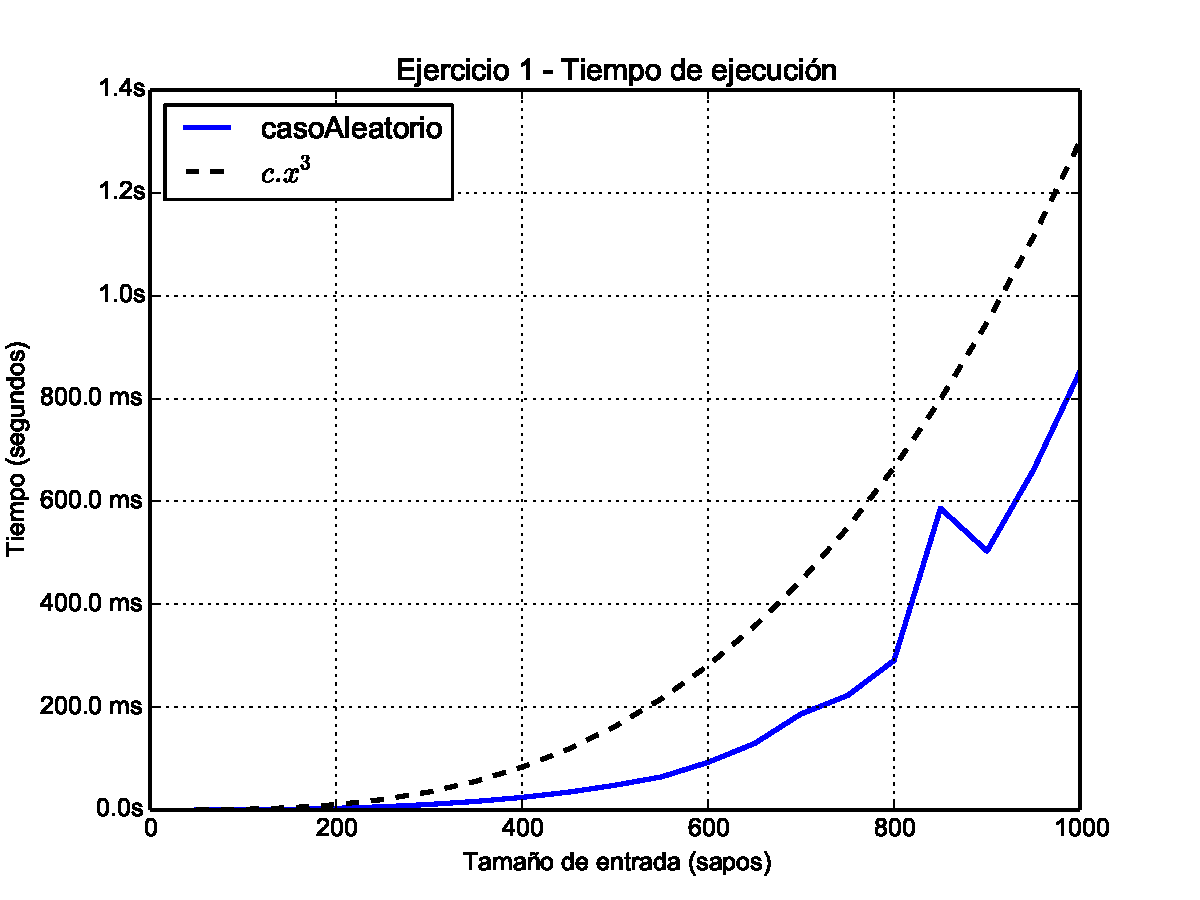
\includegraphics[width=1.4\textwidth, angle=90]{../ej1/graficos/test_tiempoLiso.pdf}
   \caption{\textbf{Muestreo general del Ejercicio 1}}
   \label{fig:ej1-graf-1}
   \end{center}
\end{figure}
\clearpage

Como conclusión, la división en casos que efectuamos no se pudo ver expresada en diferentes tiempos de ejecución.

Por otro lado, para confirmar que el algoritmo tiene una complejidad de peor caso de $\bigO{n^3}$, decidimos 
realizar un gráfico tomando el cociente $\frac{tiempoDeEjecuci\acute{o}n}{n^3}$ y variando el tamaño de entrada $n$. Usamos distribuciones aleatorias de las cartas.

Se puede apreciar que a medida que crece $n$ la curva se estabiliza muy cerca de una constante, lo que parece indicar que la cota temporal calculada fue correcta. 

%gráfico2  cociente vs n (caso peor)  
\begin{figure}[H]
   \begin{center}
   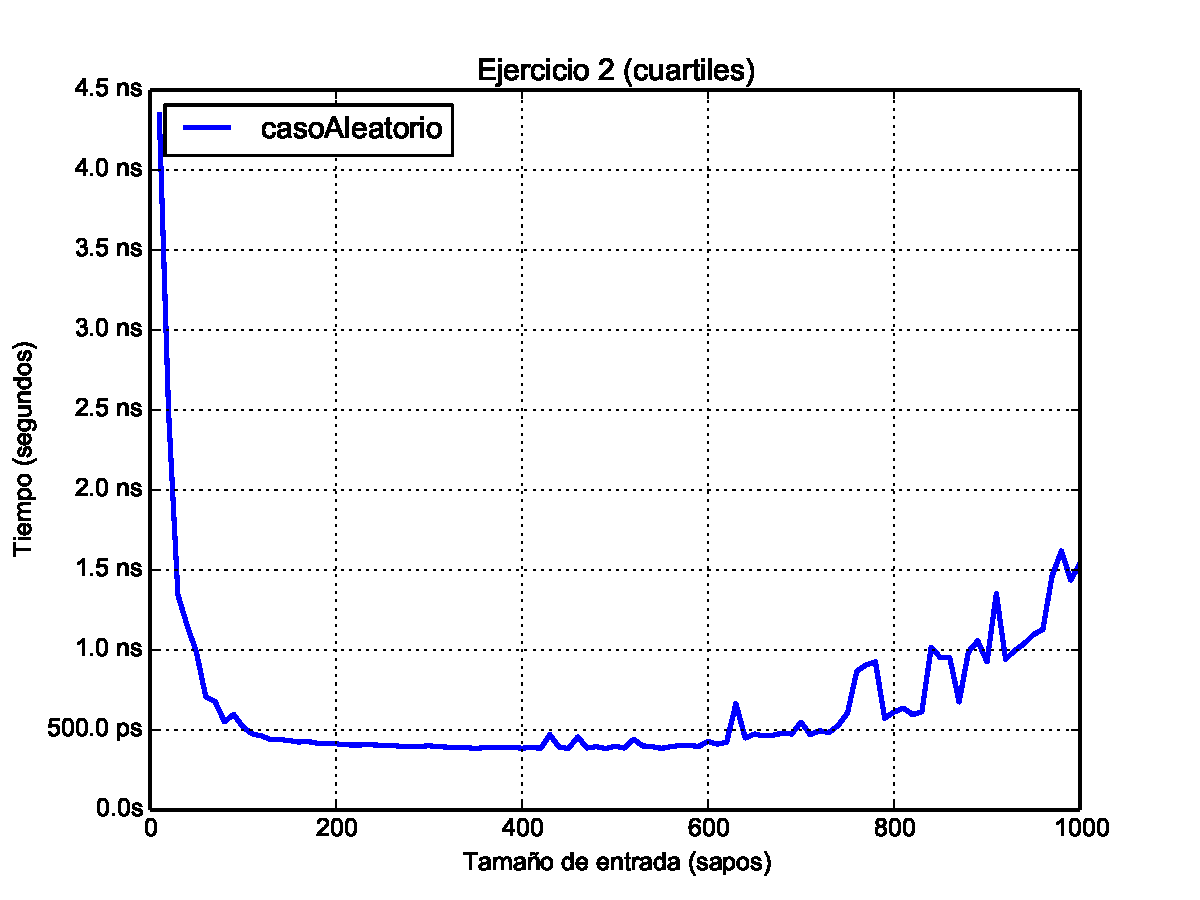
\includegraphics[width=1.4\textwidth,angle=90]{../ej1/graficos/test_division.pdf}
   \caption{\textbf{Tiempo de ejecución sobre tamaño de la entrada.}}
   \label{fig:ej1-graf-2}
   \end{center}
\end{figure}
  

\end{document}
% -----------------------------------------------
